% https://tex.stackexchange.com/a/195099
\documentclass{beamer}
\usepackage{tikz}
\usetikzlibrary{backgrounds, calc, shadows, shadows.blur}

\newcommand\addcurlyshadow[2][]{
    % #1: Optional aditional tikz options
    % #2: Name of the node to ""decorate""
    \begin{pgfonlayer}{background}
        \rotatebox{10}{%
            \path[blur shadow={shadow xshift=0pt, shadow yshift=0pt, shadow blur steps=6}, #1]
            ($(#2.north west)+(.3ex,-.5ex)$)
            -- ($(#2.south west)+(.5ex,-.7ex)$)
            .. controls ($(#2.south)!.3!(#2.south west)$) .. (#2.south)
            .. controls ($(#2.south)!.3!(#2.south east)$) .. ($(#2.south east)+(-.5ex,-.7ex)$)
            -- ($(#2.north east)+(-.3ex, -.5ex)$)
            -- cycle;
        }
    \end{pgfonlayer}
}

\begin{document}
    \begin{frame}

        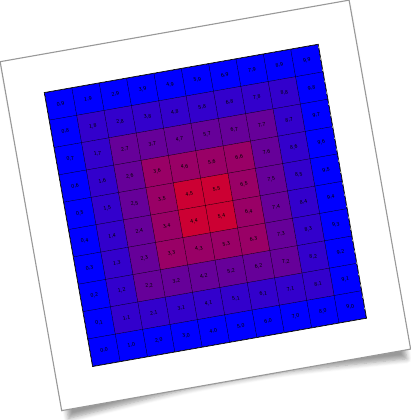
\begin{tikzpicture}

        \rotatebox{10}{%

            \node[draw=black!40, fill=white, rectangle, minimum width=4.5cm, minimum height=4.5cm]
            (example) {
                \setlength{\fboxrule}{0.2pt}%
                \setlength{\fboxsep}{0pt}%
                \fbox{%
                    \includegraphics{example-grid-100x100bp.pdf}%
                }%
            };
            \addcurlyshadow{example}
        }
        \end{tikzpicture}

    \end{frame}
\end{document}
